\documentclass{report}

\input{preamble}
\input{macros}
\input{letterfonts}

\title{\Huge{Math 120}}
\author{\huge{PSet 8}}
\date{Oct 31 2024}

\begin{document}

\maketitle
\newpage% or \cleardoublepage
% \pdfbookmark[<level>]{<title>}{<dest>}
\pdfbookmark[section]{\contentsname}{toc}
\tableofcontents
\pagebreak

\chapter{}
\section{PSet 8}

\qs{}{
    Evaluate the scalar line integral
    \[
    \int\limits_C (3x + y) \, ds,
    \]
    where \(C\) is the line segment from \((-1, 3)\) to \((4, 2)\).
}

\sol{
   \[ \int\limits_{C} (3x+y) ds \]  
   \[ (-1,3) \quad (4,2) \] 
   \[ f(t) = (1-,3) + t((4,2) - (-1, 3)) \]
   \[ f(t) = (-1,3) + t(5,-1) = \langle -1 + 5t, 3 - t\rangle \]
   \[ x = -1 + 5t \quad y = 3 - t \quad t \in  [0,1] \]
   \[ ds = \sqrt{\left(\frac{dx}{dt}\right)^{2} + \left(\frac{dy}{dt}\right)^{2}} \, dt\]   
   \[ \frac{dx}{dt} = 5 \quad \frac{dy}{dt} = - 1 \]
   \[ ds = \sqrt{5^{2} + (-1)^{2}} \, dt = \sqrt{26} \, dt \]
   \[ 3x + y \Rightarrow 3(-1+5t) + (3-t) \Rightarrow -3 + 15t + 3 - t = 14t \]
   \[ \int_{0}^{1} 14t \sqrt{26} \, dt \Rightarrow \sqrt{26} \int_{0}^{1} 14t \, dt \] 
   \[ \left. 7\sqrt{26}t^{2}\right|_{0}^{1} = 7\sqrt{26}(1)^{2} - 7\sqrt{27}(0)^{2} = 7\sqrt{26} \]     
}

\newpage 

\qs{}{
    In this problem we will sketch part of the argument that a scalar line integral \(\int_C f \, ds\) is independent of the parameterization of \(C\) that we choose to compute the integral. Suppose \(\vec{r}_1(t)\), \(a \leq t \leq b\), and \(\vec{r}_2(t)\), \(c \leq t \leq d\), are two smooth parameterizations of the same smooth curve \(C\). Assuming that both parameterizations are in the same direction it can be shown that \(\vec{r}_2(t) = \vec{r}_1(w(t))\), for some increasing function \(w(t)\) satisfying \(w(c) = a\) and \(w(d) = b\). If this is the case, show that
    \[
    \int_a^b f(\vec{r}_1(t)) \left| \vec{r}_1'(t) \right| \, dt = \int_c^d f(\vec{r}_2(t)) \left| \vec{r}_2'(t) \right| \, dt
    \]
    for any continuous function \(f\).
}

\sol{
    \[ \int\limits_{c} f \, ds \]
    \[ \vec{r_{1}}(t) \quad a \leq t \leq b \]
    \[ \vec{r_{2}}(t) \quad c \leq t \leq d \]
    \[ \vec{r_{2}}(r) = \vec{r_{1}}(w(t)) \quad w(c) = a \quad w(d) = b \] 
    \[ \int_{a}^{b} f(\vec{r_{1}}(t))|\vec{r_{1}}'(t) \, dt = \int_{c}^{d} f(\vec{r_{2}}(t))|\vec{r_{2}}'(t) \, dt \]
    \[ \vec{r_{2}}'(t) = \frac{d}{dt} \vec{r_{2}}(t) = \frac{d}{dt} \vec{r_{1}}(w(t)) = \vec{r_{1}}'(w(t)) w'(t) \]
    \[ |\vec{r_{2}}'(t)| = |\vec{r_{1}}'(w(t)) | \cdot |w'(t)| \] 
    \[ \int_{c}^{d} f(\vec{r_{2}}(t)) |\vec{r_{2}}'(t)| \, dt = \int_{a}^{b} f(\vec{r_{1}}(t)) |\vec{r_{1}}'(w(t))| \cdot |w'(t)| \, dt\]
    \[ w \text{ maps } [c, d] \text{ to } [a,b] \text{, when } t = c \, , s = a \text{, and when } t = d \, , s = b \]
    \[ \int_{a}^{b} f(\vec{r_{1}})(w(t)) |\vec{r_{1}}'(w(t))| \cdot |w(t)| \, dt = \int_{a}^{b} f(\vec{r_{1}}(s))|\vec{r_{1}}'(s)| \, ds \]
    \[ \int_{a}^{b} f(\vec{r_{1}}'(t))|\vec{r_{1}}'(t)| \, dt = \int_{a}^{b} f(r_{1}(s))|\vec{r_{1}}'(s)| \, ds = \int_{c}^{d} f(\vec{r_{2}}(t))|\vec{r_{2}}'(t)| \, dt  \] 
    $\therefore$ the scalar line integral is independent of the parameterization and the equality holds true for any continuous function f          
}

\newpage 

\qs{}{
    Sketch the vector field \(\vec{F}(x, y) = xy \, \hat{\imath} + \frac{1}{2} \, \hat{\jmath} \).
}

\sol{
    \begin{center}
        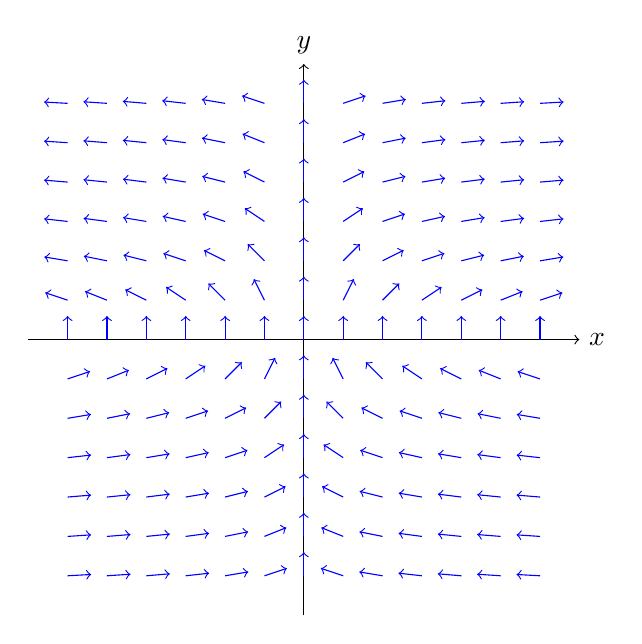
\begin{tikzpicture}[scale=1]
            % Draw axes
            \draw[->] (-3.5,0) -- (3.5,0) node[right] {$x$};
            \draw[->] (0,-3.5) -- (0,3.5) node[above] {$y$};
          
            % Loop over grid points
            \foreach \x in {-3,-2.5,...,3}
            \foreach \y in {-3,-2.5,...,3}
            {
              % Calculate vector components
              \pgfmathsetmacro{\u}{\x*\y}
              \pgfmathsetmacro{\v}{0.5}
          
              % Normalize vector length for consistent arrow sizes
              \pgfmathsetmacro{\len}{sqrt((\u)^2+(\v)^2)}
              \pgfmathsetmacro{\unorm}{\u/\len*0.3}
              \pgfmathsetmacro{\vnorm}{\v/\len*0.3}
          
              % Draw vector arrow
              \draw[->, blue] (\x,\y) -- +(\unorm,\vnorm);
            }
          \end{tikzpicture}
    \end{center}
}

\qs{}{
    Given the contour diagram for a function \(f\) shown below, in which dark colors correspond to low values of \(f\) and light colors correspond to high values of \(f\), sketch the gradient vector field \(\vec{F} = \nabla f\).
    \insertpng[0.25]{prob4.png}
}

\sol{
    \begin{center}
        \insertpng[0.05]{prob4ans.png}
    \end{center}
}
\qs{}{
    A thin wire has the shape of the curve \(C\) parameterized by \(x = \cos t\), \(y = \sin t\), \(z = t\), \(0 \leq t \leq 4\pi\), where \(x, y,\) and \(z\) are measured in centimeters. The linear density of the wire is given by \(\rho(x, y, z) = x^2 z\) grams per centimeter. Find the mass of the wire.
}

\sol{
    \[ x = \cos t \quad y = \sin t \quad z = t \]
    \[ 0 \leq t \leq 4\pi \] 
    \[ \rho(x,y,x) = x^{2}z \frac{\text{grams}}{\text{cm}} \] \
    \[ \text{Mass: } = \int\limits_{C} \rho(x,y,z) ds \] 
    \[ \frac{dx}{dt} = - \sin t \quad \frac{dy}{dt} = \cos t \quad \frac{dz}{dt} = 1 \] 
    \[ ds = \sqrt{\left(\frac{dx}{dt}\right)^{2} + \left(\frac{dy}{dt}\right)^{2} + \left(\frac{dz}{dt}\right)^{2} } \, dt \] 
    \[ ds = \sqrt{\left(-\sin(t)\right)^{2} + \left(\cos (t)\right)^{2} + \left(1\right)^{2} } \, dt \]  
    \[ ds = \sqrt{1 + 1} \, dt = \sqrt{2} \, dt \] 
    \[ \rho(x,y,z) = x^{2}z \Rightarrow \cos^{2}t \cdot t \Rightarrow t \cos^{2} t \]
    \[ \text{Mass: } \int_{0}^{4\pi} \rho(t) ds = \int_{0}^{4\pi} t \cos^{2} t \sqrt{2} \, dt \]
    \[ \sqrt{2} \int_{0}^{4} t \cos ^{2} t dt \quad \cos^{2}t = \frac{1 + \cos 2t}{2} \] 
    \[ \sqrt{2} \int_{0}^{4\pi} t \left(\frac{1 + \cos 2t}{2}\right) \, dt \Rightarrow \frac{\sqrt{2}}{2} \int_{0}^{4\pi} t (1 + \cos 2t )\, dt \]
    \[ \frac{\sqrt{2}}{2} \int_{0}^{4\pi} t \, dt + \frac{\sqrt{2}}{2} \int_{0}^{4\pi} t \cos 2t \, dt \] 
    \[ \int_{0}^{4\pi} t \, dt = \left. \frac{t^{2}}{2}\right|_{0}^{4\pi} \Rightarrow \frac{\sqrt{2}}{2} \frac{16 \pi^{2}}{2} - \frac{\sqrt{2}}{2} \frac{0}{2} = 4\sqrt{2}\pi^{2} \] 
    \[ u = t \quad du = dt \]
    \[ v = \frac{1}{2} \sin 2t \quad dv = \cos 2t \]
    \[ \int t \cos 2t \, dt = t \cdot \frac{1}{2} \sin 2t - \int \frac{1}{2} \sin 2t dt = \frac{1}{2} t \sin 2t + \frac{1}{4} \cos 2t + k \]
    \[ \left[ \frac{1}{2} t \sin 2t + \frac{1}{4} \cos 2t \right]_{0}^{4 \pi} = \left( \frac{1}{2} \cdot 4 \pi \cdot 0 + \frac{1}{4} \cdot 1 \right) - \left(0 + \frac{1}{4} \cdot 1\right) = 0 \]
    \[ 4 \sqrt{2} \pi^{2} + 0 = 4 \sqrt{2}\pi^{2} \]       
}

\newpage 

\qs{}{
    Let \(\vec{F}\) be the vector field shown below, and let \(C\) be the unit circle, oriented clockwise. Is the vector line integral
    \[
    \int_C \vec{F} \cdot d\vec{r}
    \]
    positive, negative, or zero? Explain your reasoning.
    \insertpng[0.25]{prob6.png}
}

\sol{ 
    \\
    The vector field is in the same direction as C, so it is positive. 
}

\qs{}{
    Evaluate the line integral 
    \[
    \int_C \sin x \, dx + \cos y \, dy
    \]
    where \(C\) consists of the top half of the circle \(x^2 + y^2 = 1\) from \((1, 0)\) to \((-1, 0)\) and the line segment from \((-1, 0)\) to \((-2, 3)\). (Remember that when you see an integral that looks like 
    \[
    \int_C P(x, y) \, dx + \int_C Q(x, y) \, dy
    \]
    it is a shorthand notation for 
    \[
    \int_C \vec{F}(\vec{r}(t)) \cdot d\vec{r}
    \]
    where \(\vec{F}(x, y) = \langle P(x, y), Q(x, y) \rangle\). The analogous thing is true in three dimensions.)
}

\sol{
    \[
    x^{2} + y^{2} = 1 \quad x = \cos t \quad y = \sin t \quad t \in [0, \pi]
    \]

    \[
    x(t) = (1 - t)(-1) + t(-2) \quad y(t) = (1 - t)(0) + t(3) \quad t \in [0,1]
    \]

    \[
    \vec{F}(x, y) = \langle \sin x, \cos y \rangle
    \]

    \[
    \int\limits_{C} \sin x \, dx + \cos y \, dy
    \]

    \[ 
    x(t) = \cos t, \quad y(t) = \sin t, \quad t \in [0, \pi]
    \]

    \[
    \frac{dx}{dt} = -\sin t, \quad \frac{dy}{dt} = \cos t
    \]

    \[
    \int\limits_{C_1} \sin x \, dx + \cos y \, dy = \int_{0}^{\pi} \left[ \sin(\cos t)(- \sin t) + \cos(\sin t) \cos t \right] dt
    \]

    \[
    \int_{0}^{\pi} \sin(\cos t)(- \sin t) \, dt + \int_{0}^{\pi} \cos(\sin t) \cos t \, dt
    \]

    \[
    f(x, y) = -\cos x + \sin y
    \]

    At \((1, 0)\):
    \[
    f(1, 0) = -\cos(1) + \sin(0) = -\cos(1)
    \]

    At \((-1, 0)\):
    \[
    f(-1, 0) = -\cos(1)
    \]

    \[
    \int\limits_{C_1} \sin x \, dx + \cos y \, dy = f(-1, 0) - f(1, 0) = 0
    \]

    \[
    x(t) = -1 - t, \quad y(t) = 3t, \quad t \in [0, 1]
    \]

    \[
    dx = -1 \, dt, \quad dy = 3 \, dt
    \]

    \[
    \int\limits_{C_2} \sin x \, dx + \cos y \, dy = \int_{0}^{1} \left[ \sin(-1 - t)(-1) + \cos(3t)(3) \right] dt
    \]


    Using \(\sin(-1 - t) = -\sin(1 + t)\), the integral becomes:
    \[
    \int_{0}^{1} \sin(1 + t) \, dt + 3 \int_{0}^{1} \cos(3t) \, dt
    \]

    \[
    \int_{0}^{1} \sin(1 + t) \, dt = -\cos(1 + t) \Big|_0^1 = -\cos(2) + \cos(1)
    \]

    \[
    3 \int_{0}^{1} \cos(3t) \, dt = 3 \left( \frac{1}{3} \sin(3t) \Big|_0^1 \right) = \sin(3)
    \]

    \[
    \int\limits_{C_2} \sin x \, dx + \cos y \, dy = \cos(1) - \cos(2) + \sin(3)
    \]

    \[
    \int\limits_{C} \sin x \, dx + \cos y \, dy = \int\limits_{C_1} \sin x \, dx + \cos y \, dy + \int\limits_{C_2} \sin x \, dx + \cos y \, dy
    \]

    Since \( \int\limits_{C_1} \sin x \, dx + \cos y \, dy = 0 \), the total integral is:
    \[
    \int\limits_{C} \sin x \, dx + \cos y \, dy = \cos(1) - \cos(2) + \sin(3)
    \]

}

\newpage

\qs{}{
    Compute the line integral of the vector field 
    \[
    \vec{F}(x, y) = \frac{x}{\sqrt{x^2 + y^2}} \hat{\imath} + \frac{y}{\sqrt{x^2 + y^2}} \hat{\jmath}
    \]
    along the parabola \(x = 1 + y^2\) from \((2, -1)\) to \((2, 1)\).
}

\sol{
    \[ \int\limits_{C} \vec{F} \cdot d\vec{r} = \int_{a}^{b} \left[ F_{1} (x(t),y(t)) \frac{dx}{dt} + F_{2}(x(t), y(t)) \frac{dy}{dt} \right] dt \] 
    \[ y = t \quad t \in [-1,1] \quad x(t) = 1 + t^{2} \]
    \[ r(t) = \langle x(t), y(t) \rangle = \langle 1 + t^{2}, t \rangle \quad t \in [-1,1] \] 
    \[ \frac{dx}{dt} = 2t \quad \frac{dy}{dt} = 2 \] 
    \[ \vec{F}(x,y) \Rightarrow \vec{F}(1 + t^{2}, t) =  \frac{1+t^{2}}{\sqrt{\left(1+t^{2}\right)^{2} + t^{2}}} \hat{\imath} +  \frac{t}{\sqrt{\left(1+t^{2}\right)^{2} + t^{2}}} \hat{\jmath} \]
    \[ \left[ \frac{1+t^{2}}{\sqrt{\left(1+t^{2}\right)^{2} + t^{2}}} \times 2t \right] + \left[ \frac{t}{\sqrt{\left(1+t^{2}\right)^{2} + t^{2}}} \times 1 \right] \]
    \[ \int_{a}^{b} \left[ \frac{3t+2t^{3}}{\sqrt{\left(1+t^{2}\right)^{2} + t^{2}}}\right] dt \]
    \[ \int_{a}^{b} \frac{3t+2t^{3}}{\sqrt{1+3t^{2}+t^{4}}} dt \]
    \[ d\vec{r} = (2t \hat{\imath}, 2 \hat{\jmath})\] 
    \[ \vec{F} \cdot d\vec{r} = \frac{3t+2t^{3}}{\sqrt{1+3t^{2}+t^{4}}} \]
    \[ d\frac{d}{dt} \sqrt{1 + 3t^{2} + t^{4}} = \frac{3t + t^{2}}{\sqrt{t^{4} + 3t^{2} + 1}} \] 
    \[ \vec{F} \cdot d\vec{r} = d\left( \sqrt{t^{4} + 3t^{2} + 1} \right)\] 
    \[ \int_{a}^{b} \vec{F} d\vec{r} = \left[ t^{4} + 3t^{2} + 1 \right]_{-1}^{1} = \sqrt{1^{4} + 3(1)^{2} + 1 } - \sqrt{1 + 3(-1)^{2} + (-1)^{4}} = 0 \] 
}

\qs{}{
    Evaluate the line integral of the vector field
    \[
    \vec{F}(x, y, z) = (x + y) \hat{\imath} + (y - z) \hat{\jmath} + z^2 \hat{k}
    \]
    along the path parameterized by 
    \[
    \vec{r}(t) = t^2 \hat{\imath} + t^3 \hat{\jmath} + t^2 \hat{k}, \quad 0 \leq t \leq 1.
    \]
}
\sol{
    \[ \vec{F}(x,y,x) = (x + y) \hat{\imath} + (y - z) \hat{\jmath} + z^2 \hat{k} \] 
    \[ \vec{r}(t) = t^2 \hat{\imath} + t^3 \hat{\jmath} + t^2 \hat{k}, \quad 0 \leq t \leq 1 \]
    \[ \frac{d\vec{r}}{dt} = 2t \, \hat{\imath} + 3t^{2} \hat{\jmath} + 2t \, \hat{k} \]
    \[ \vec{F}(t) = \left[ t^{2} + t^{3} \right] \, \hat{\imath} + \left[ t^{3} - t^{2} \right] \, \hat{\jmath} + \left[ t^{4} \right] \, \hat{k} \]
    \[ \vec{F} \cdot \frac{dr}{dt} = \left[ \left(t^{2} + t^{3} \right)(2t) \right] + \left[ \left(t^{2} - t^{3} \right)\left(3t^{2}\right) \right] + \left[ \left(t^{4}\right)(2t)\right]\]   
    \[ \vec{F} \frac{d\vec{r}}{dt} = 2t^{3} - t^{4} + 5t^{5} \]
    \[ \int_{0}^{1} \left[ 2t^{3} - t^{4} + 5t^{5} \right] dt = \left[ \frac{1}{2}t^- \frac{1}{5}t^{5} + \frac{5t^{6}}{6} \right]_{0}^{1} \]\
    \[ \left( \frac{1}{2} - \frac{1}{5} + \frac{5}{6} \right) - 0 = \frac{17}{15} \]   
}

\newpage 

\qs{}{
    For each of the following vector fields \(\vec{F}\) and curves \(C\), find a function \(f\) such that \(\vec{F} = \nabla f\) and use this function to evaluate 
    \[
    \int_C \vec{F} \cdot d\vec{r}
    \]
    along the given directed curve \(C\).
    \begin{enumerate}
        \item \(\vec{F}(x, y) = \langle x^2, y^2 \rangle\),  
        \(C\) is the arc of the parabola \(y = 2x^2\) from \((-1, 2)\) to \((2, 8)\).

        \item \(\vec{F}(x, y, z) = \langle e^y, xe^y, (z + 1)e^z \rangle\),  
        \(C : \vec{r}(t) = \langle t, t^2, t^3 \rangle\), \(0 \leq t \leq 1\).
    \end{enumerate}
}

\sol{
    \[ F = \nabla f \]
    \[ \int\limits_{C} F \cdot d\vec{r} = f(\text{end point}) - f(\text{start point}) \] 
    Problem 1 
    \[ \frac{\partial f}{\partial x} = x^{2} \quad \frac{\partial f}{\partial y} = y^{2} \]
    \[ f(x,y) = \int x^{2} \, dx = \frac{1}{3}x^{2} + g(y) \]
    \[ \frac{\partial g}{\partial y} = g'(y) = y^{2} \]
    \[ g(y) = \int_ y^{2} \, dy = \frac{1}{3}y^{3} \]
    \[ f(x,y) = \frac{1}{3}x^{3} + \frac{1}{3}y^{3} \]
    \[ \int F \, d\vec{r} = f(2,8) - f(-1,2) = 171 \] 
    Problem 2
    \[ \vec{F}(x,y,z) = \langle e^{y}, xe^{y}, (z + 1)e^{z} \rangle \quad \vec{r}(t) = \left(t,t^{2}, t^{3}\right) \]    
    \[ \frac{\partial F}{x} = e^{x} \quad \frac{\partial F}{\partial y} = xe^{y} \quad \frac{\partial F}{\partial z} = (z+1)e^{z} \] 
    \[ f(x,y,z) = \int e^{y} \, dx = xe^{y} + \rho(y,z) \]
    \[ \frac{\partial f}{\partial y} = xe^{y} + \frac{\partial \rho}{\partial y} \quad xe^{y} + \frac{\partial \rho}{\partial y} \quad \frac{\partial \rho}{\partial y} = 0 \]
    \[ \rho(x,y,z) = \phi(z) \]
    \[ \frac{\partial f}{\partial z} = (z+1)e^{z} \]
    \[ \rho(z) = \int (z+1)e^{z} \, dz \]
    \[ u = z + 1 \quad du = 1 \, dz \] 
    \[ v = e^{z} \, dv = e^{z} \, dz \] 
    \[ \int (z+1)e^{z} \, dz = (z+1) e^{z} - \int e^{z} \, dz \] 
    \[ (z+1)e^{z} - e^{z} \Rightarrow ze^{z} + e^{z} - e^{z} = ze^{z} \]
    \[ f(x,y,z) = xe^{y} + ze^{z} \]
    \[ f(1,1,1) = (1)e^{1} + (1)e^{1} = ze \] 
    \[ f(0,0,0) = (0)e^{0} + + (0)e^{0} = 0 \]
    \[ \int\limits_{C} \vec{F} \cdot d\vec{r} = f(1,1,1) - f(0,0,0) = 2e \]          
}

\qs{}{
    Clairaut's Theorem implies that if the vector field \(\vec{F} = P \hat{\imath} + Q \hat{\jmath} + R \hat{k}\) is conservative and \(P, Q,\) and \(R\) have continuous first-order partial derivatives, then
    \[
    \frac{\partial P}{\partial y} = \frac{\partial Q}{\partial x}, \quad 
    \frac{\partial P}{\partial z} = \frac{\partial R}{\partial x}, \quad 
    \frac{\partial Q}{\partial z} = \frac{\partial R}{\partial y}.
    \]
    \begin{enumerate}
        \item Use the statement above to show that the vector line integral
        \[
        \int_C x \, dx + 2x \, dy + xz \, dz
        \]
        is not independent of path.

        \item Find two directed curves \(C_1\) and \(C_2\) that start at the same point and end at the same point, such that
        \[
        \int_{C_1} x \, dx + 2x \, dy + xz \, dz \neq \int_{C_2} x \, dx + 2x \, dy + xz \, dz.
        \]
    \end{enumerate}
}

\sol{ 
    \\
    a) 
    \[
    \frac{\partial P}{\partial y} = \frac{\partial Q}{\partial x}, \quad 
    \frac{\partial P}{\partial z} = \frac{\partial R}{\partial x}, \quad 
    \frac{\partial Q}{\partial z} = \frac{\partial R}{\partial y}.
    \]

    \[
    P = x, \quad Q = 2x, \quad R = xz.
    \]

    \[
    \frac{\partial P}{\partial y} = \frac{\partial x}{\partial y} = 0, \quad 
    \frac{\partial Q}{\partial x} = \frac{\partial 2x}{\partial x} = 2.
    \]

    \[
    \frac{\partial P}{\partial z} = \frac{\partial x}{\partial z} = 0, \quad 
    \frac{\partial R}{\partial x} = \frac{\partial (xz)}{\partial x} = z.
    \]

    \[
    \frac{\partial Q}{\partial z} = \frac{\partial 2x}{\partial z} = 0, \quad 
    \frac{\partial R}{\partial y} = \frac{\partial (xz)}{\partial y} = 0.
    \]

    The first inequality does not hold true nor does teh second but third does. This means that it is not conservative \\

    b) 
    \[
    \int_C x \, dx + 2x \, dy + xz \, dz
    \]

    \[
    A = (0, 0, 0), \quad B = (1, 0, 0)
    \]

    \[
    x = t, \quad y = 0, \quad z = 0, \quad t \in [0, 1]
    \]

    \[
    dx = dt, \quad dy = 0, \quad dz = 0
    \]

    \[
    \int_{C_1} x \, dx + 2x \, dy + xz \, dz = \int_{0}^{1} t \, dt = \left[ \frac{1}{2} t^2 \right]_0^1 = \frac{1}{2}
    \]

    \[
    C_2: \quad C_{2a}, \quad C_{2b}, \quad C_{2c}
    \]

    \[
    C_{2a}: \quad (0, 0, 0) \to (0, 1, 0)
    \]

    \[
    x = 0, \quad y = t, \quad z = 0, \quad t \in [0, 1]
    \]

    \[
    dx = 0, \quad dy = dt, \quad dz = 0
    \]

    \[
    \int_{C_{2a}} x \, dx + 2x \, dy + xz \, dz = \int_{0}^{1} 0 \, dt = 0
    \]

    \[
    C_{2b}: \quad (0, 1, 0) \to (1, 1, 0)
    \]

    \[
    x = t, \quad y = 1, \quad z = 0, \quad t \in [0, 1]
    \]

    \[
    dx = dt, \quad dy = 0, \quad dz = 0
    \]

    \[
    \int_{C_{2b}} x \, dx + 2x \, dy + xz \, dz = \int_{0}^{1} t \, dt = \left[ \frac{1}{2} t^2 \right]_0^1 = \frac{1}{2}
    \]

    \[
    C_{2c}: \quad (1, 1, 0) \to (1, 0, 0)
    \]

    \[
    x = 1, \quad y = t, \quad z = 0, \quad t \in [1, 0]
    \]

    \[
    dx = 0, \quad dy = dt, \quad dz = 0
    \]

    \[
    \int_{C_{2c}} x \, dx + 2x \, dy + xz \, dz = 2 \int_{1}^{0} dt = 2 (0 - 1) = -2
    \]

    \[
    \int_{C_2} = \int_{C_{2a}} + \int_{C_{2b}} + \int_{C_{2c}} = 0 + \frac{1}{2} + (-2) = -\frac{3}{2}
    \]

    \[
    \int_{C_1} x \, dx + 2x \, dy + xz \, dz = \frac{1}{2}
    \]

    \[
    \int_{C_2} x \, dx + 2x \, dy + xz \, dz = -\frac{3}{2}
    \]

    \[
    \frac{1}{2} \neq -\frac{3}{2}
    \]

    \[
    \int_{C_1} x \, dx + 2x \, dy + xz \, dz \ne \int_{C_2} x \, dx + 2x \, dy + xz \, dz
    \]

}

\newpage 

\qs{}{
    The force exerted by an electric charge at the origin on a charged particle at a point \((x, y, z)\) with position vector \(\vec{r} = \langle x, y, z \rangle\) is 
    \[
    \vec{F}(\vec{r}) = K \frac{\vec{r}}{|\vec{r}|^3},
    \]
    where \(K\) is a constant. Find the work done on the particle as it moves along the straight line from \((0, 3, 0)\) to \((1, 3, 2)\) in two ways:
    \begin{enumerate}
        \item Parameterize the line segment, and compute 
        \[
        \int_a^b \vec{F}(\vec{r}(t)) \cdot \vec{r}'(t) \, dt
        \]
        directly.
        
        \item Although \(\vec{F}\) is not defined at the origin, it turns out that \(\vec{F}\) is conservative on its domain. Find a potential function \(f\), and use the Fundamental Theorem of Line Integrals to compute the work done on the particle.
    \end{enumerate}
}

\sol{
    \\
    a) 
    \[
    \vec{r}(t) = (t, 3, 2t), \quad t \in [0, 1]
    \]
    \[
    \vec{r}'(t) = \langle 1, 0, 2 \rangle
    \]
    \[
    |\vec{r}(t)| = \sqrt{5t^2 + 9}
    \]
    \[
    \vec{F}(\vec{r}(t)) = K \frac{\langle t, 3, 2t \rangle}{(5t^2 + 9)^{3/2}}
    \]
    \[
    \vec{F}(\vec{r}(t)) \cdot \vec{r}'(t) = K \frac{5t}{(5t^2 + 9)^{3/2}}
    \]
    \[
    W = \int_0^1 K \frac{5t}{(5t^2 + 9)^{3/2}} \, dt
    \]
    Substitution: \( u = 5t^2 + 9 \), \( du = 10t \, dt \)
    \[
    W = K \int_9^{14} \frac{du}{2u^{3/2}}
    \]
    \[
    W = \frac{K}{2} \int_9^{14} u^{-3/2} \, du
    \]
    \[
    W = -K \left[ u^{-1/2} \right]_9^{14} = K \left( \frac{1}{3} - \frac{1}{\sqrt{14}} \right)
    \]

    b) 
    \[
    f(\vec{r}) = -\frac{K}{|\vec{r}|}
    \]
    \[
    W = f(\vec{r}_B) - f(\vec{r}_A)
    \]
    \[
    |\vec{r}_A| = 3, \quad |\vec{r}_B| = \sqrt{14}
    \]
    \[
    W = K \left( \frac{1}{3} - \frac{1}{\sqrt{14}} \right)
    \]
}

\end{document}